%%=============================================================================
%% Methodologie
%%=============================================================================

\chapter{\IfLanguageName{dutch}{Methodologie}{Methodology}}%
\label{ch:methodologie}

%% Maak voor elke fase (behalve het literatuuronderzoek) een NIEUW HOOFDSTUK aan
%% en geef het een gepaste titel.

\begin{figure*}
    \centering
    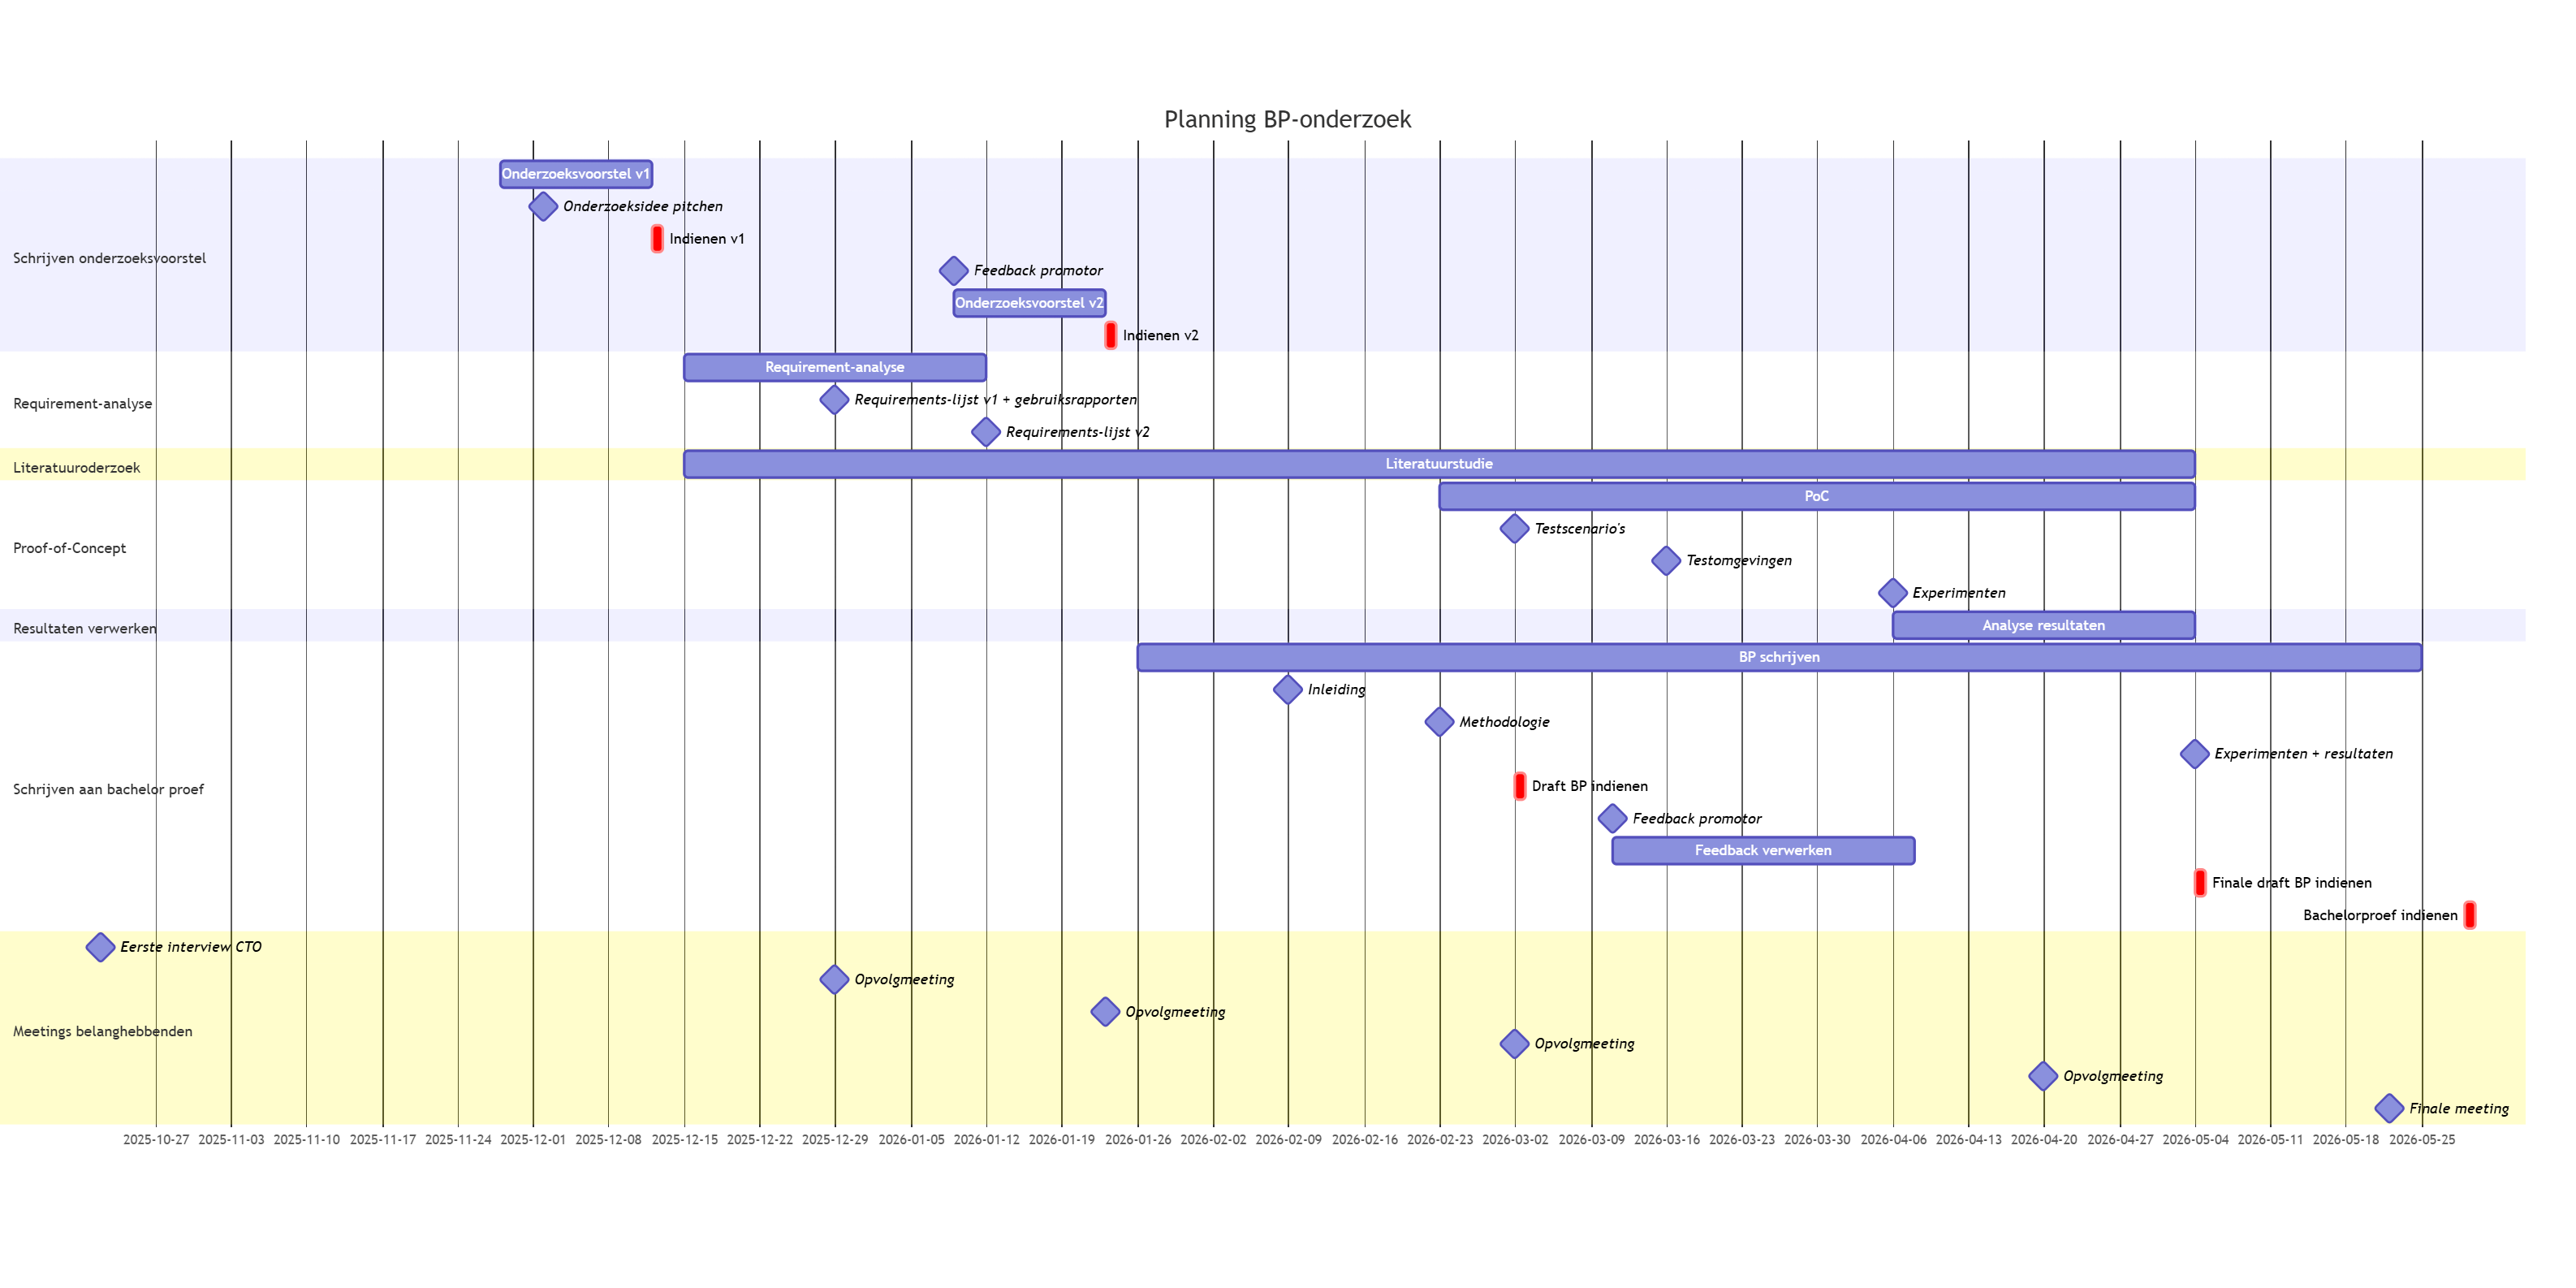
\includegraphics[width=\textwidth]{../graphics/GanttPlanningBP}
    \caption[Fases en milestones onderzoek]{Gantt diagram met de verschillende fases en milestones van het onderzoek.}
\end{figure*}

Deze studie werd op een iteratieve manier uitgevoerd. Er werd op regelmatige basis feedback gevraagd en verwerkt van de belanghebbenden en promotor. Tijdens het uitvoeren van dit onderzoek ging er ook tijd naar het schrijven van een onderzoeksvoorstel en bachelorproef. Bij de planning werd uitgegaan van 8 uur werk per week zonder rekening te houden met eventuele vakanties, weekends en feestdagen.

\section{Fase 1: Requirements-analyse}

Het onderzoek startte met een requirements-analyse. De functie in het probleemdomein werd onderworpen aan een eerste analyse, waaruit een requirements-lijst ontstond. Samen met de co-promotor werd deze lijst besproken en verder gefinaliseerd om de verwachtingen en richting van het onderzoek te bepalen. Op het einde van deze fase was er een lijst van eisen die kon dienen als basis om de literatuurstudie op te starten. Daarnaast werd er ook een antwoord gevonden op de volgende deelvragen: 

\begin{itemize}
    \item Wat zijn de beperkingen van de huidige toepassing?
    \item Wat maakt de bestaande applicatie dynamisch en seizoensgebonden? 
    \item Welke architecturale en technische factoren zijn belangrijk bij de huidige toepassing? 
    \item Aan welke eisen moet een nieuwe oplossing voldoen om als succesvol aanzien te worden?
\end{itemize}

De tijdsduur die nodig was in deze fase was 32 uur verspreid over 4 weken.

\section{Fase 2: Literatuurstudie}

In de volgende stap werd er op basis van de requirements-lijst uit de vorige fase een longlist opgesteld die alle potentiële alternatieven in kaart bracht. Deze lijst werd wederom besproken met de co-promotor. Uit dit gesprek kwam de beslissing om voornamelijk te focussen op containergebaseerde oplossingen wat resulteerde in een shortlist van Azure Container Apps en Google Cloud Run. Uiteindelijk werd er een uitgebreide literatuurstudie uitgevoerd op het probleemdomein en de technologieën uit de shortlist. Deze studie gaf bepaalde inzichten die later konden gebruikt worden bij de vergelijking van deze technologieën. Er kwam een antwoord op de volgende deelvraag: 

\begin{itemize}
    \item Wat zijn de belangrijkste technische verschillen tussen de mogelijke oplossingen?
\end{itemize}

Deze fase heeft 80 uur in beslag genomen over een periode van 20 weken. 

\section{Fase 3: Proof-of-Concept}

Vervolgens kon de Proof-of-Concept opgestart worden. Hierbij werden de testomgevingen in Azure en Google Cloud opgezet en werd ook de dynamische functie in een container gestoken a.d.h.v. een Dockerfile. Op deze manier kon de functie in een container draaien zonder platformspecifieke kenmerken te moeten implementeren. Het garandeerde ook dat zowel het probleemdomein als de mogelijke alternatieven op een objectieve manier met elkaar vergeleken konden worden. Deze stappen en configuraties werden gedocumenteerd, zodat dit later kon opgenomen worden in een stappenplan. Er kwam een antwoord op de deelvragen: 

\begin{itemize}
    \item Wat zijn de architecturale overwegingen en uitdagingen bij een migratie naar een andere oplossing?
    \item Welke stappen dienen er genomen te worden bij een migratie naar de mogelijke oplossingen?
    \item Hoeveel tijd neemt een migratie naar de mogelijke oplossingen in beslag?
\end{itemize}

In de volgende stap van deze fase werden relevante testscenario's uitgewerkt en uitgevoerd op de verschillende omgevingen. De testen werden geautomatiseerd door middel van Python, waarbij variabelen gedefinieerd werden op één plaats. Er werd gekeken naar de prestaties en schaalbaarheid van elke toepassing. Concreet werden de volgende criteria onder de loep genomen:

\begin{itemize}
    \item cold start tijd
    \item gemiddelde afhandelingstijd
    \item Doorvoersnelheid (aanvraag/seconde)
    \item CPU-gebruik
    \item Geheugengebruik
\end{itemize}

Deze informatie werd verkregen via Application Insight en bijgehouden in een Excel om een verdere analyse op uit te voeren. Elke benchmark werd minstens 30 keer uitgevoerd per testomgeving, zodat er een normaal verdeling was van de gemiddelden\footnote{centrale limietstelling}. Om de kosten te berekenen, werden prijzencalculators van de verschillende cloud providers gebruikt. Als eindresultaat van deze fase waren de nodige gegevens beschikbaar waarop het advies gebaseerd kon worden, alsook alle scripts die het automatiseren van de benchmarks mogelijk maken. De tijd die hiervoor nodig was, was 80 uur verspreid over 10 weken.

\section{Fase 4: Resultaten}

Tot slot werd er een analyse op de resultaten uitgevoerd door de gemiddeldes, medianen, standaarddeviaties, minimale/maximale waarden en spreiding van de resultaten te berekenen. Deze afgeleide data werd vervolgens gebruikt om statistische testen op uit te voeren. Hierbij werd gekeken naar een afhankelijke (resultaten) en een onafhankelijke (cloud provider) variabele. Deze bevindingen werden gevisualiseerd met Python en gaven een antwoord op de deelvragen: 

\begin{itemize}
    \item Welke impact heeft een migratie naar de mogelijke oplossingen?
    \item Wat is de superieure oplossing?
\end{itemize}

 Aan de hand van deze analyse, het stappenplan van de migratie en de tijdsinschatting hiervan, werd er een advies opgesteld. Hierop kunnen de belanghebbenden zich baseren om een beslissing te nemen. Deze conclusie nam ongeveer 32 uur in beslag verspreid over 4 weken. 